\documentclass[document.tex]{subfiles}

\begin{document}

\chapter{Methodology}

\section{Introduction}
\noindent \textbf{Percentage word problem solver (PWPS)} is the system to solve percentage word problems with the help of ALGES which is a step towards solving math word problems automatically. It first converts the problem text to usable in ALGES, generates equations, train local model and global model and finally predict the solution. We discussed the system in details in the following sections.

In our system, we have used ALGES to a broader scope to solve percentage word problems. We have converted the problem text first. Then generate equation trees by semantic parsing and \textbf{Integer Linear Programming (ILP)} to solve the problem. 

In training, we train local relationship model from the generated equations and their results to set an operator between two operands and a global model based on the equations solution label by correct or incorrect. 

In testing, set a score for the generated equations from the local and global model and choose the equation with the highest score as the final equation for a problem text.

\section{Flowchart of PWPS} Percentage Word Problem Solver (PWPS) starts with the problem text and its solution. Then it divides based on the test or train categories. Flowchart for PWPS is shown in Figure \ref{fig:flowchart} which gives the overview of our proposed system. 
\begin{figure}[H]
	\begin{center}
\begin{tikzpicture}[node distance=1.2cm]
% Place nodes
\node [startstop] (init) {START};
\node [io,  below of=init] (input) {Problem Text, $p$};
\node [process, below of = input] (convert) {Convert to Fraction};
\node [process, below of= convert] (ground) {Ground \& Tokenize $p$ };
\node [process, below of=ground] (tree) {Generate Tree $T(p)$};
\node [decision, below of= tree, node distance=3cm] (tt){Test or Train};
\node [process, left of = Ev, below of=tt,node distance=3cm] (TrLocal){Train Local};
\node [process, below of=TrLocal, node distance=1.5cm] (TrGlobal){Train Global};
\node [process, right of=TrLocal, node distance=6cm] (Ev){Evaluate};
\node [process, right of=TrGlobal, node distance=6cm] (Sol){Solution};
\node [startstop, below of = tt, node distance = 6cm] (st){STOP};

% Draw edges
\draw [arrow] (init) -- (input);
\draw [arrow] (input) -- (convert);
\draw [arrow] (convert) -- (ground);
\draw [arrow] (ground) -- (tree);
\draw [arrow] (tree) -- (tt);
\draw [arrow] (tt) -| node[anchor=north west]{Train}(TrLocal);
\draw [arrow] (TrLocal) --(TrGlobal);
%\draw [arrow] (TrGlobal)-|node[anchor=north west]{Train}(st);
\draw [arrow] (tt)-|node[anchor=north east]{Test}(Ev);
\draw [arrow] (Ev)--(Sol);
\draw [arrow] (Sol)|-(st);
\draw [arrow] (TrGlobal) |- (st);
\end{tikzpicture}
\end{center}
\caption{Flowchart of PWPS}
\label{fig:flowchart}
\end{figure}
\noindent It firstly take the problem text as input that is a string, then passes through the converting portion. After equation generating, there is two-phase. One is training phase, and another is testing phase. 

All the training steps in the algorithm are discussed in this paper as \textbf{“Learning”}, and testing steps are discussed as \textbf{“Inference”}. 

Learning contains train local and global model, and inference contains equation evaluation and solution checking concerning the actual solution of the problem text. Algorithm for PWPS is given in the Figure \ref{fig:algo}.

\section{Algorithm of PWPS}
Algorithm of Percentage Word Problem Solver (PWPS) consists of two part. One is ``Learning" and the other is ``Inference".
\begin{figure}[H]
	\begin{algorithm}[H]
		\caption{: \textbf{Learning}}
		\begin{algorithmic}[1]
			\renewcommand{\algorithmicrequire}{\textbf{Input:}}
			\renewcommand{\algorithmicensure}{\textbf{Output:}}
			\REQUIRE Problem Text, P and Solution, l
			\ENSURE  Local Model $\mathcal{L}_{local}$, Global Model $ \mathcal{G}{global}$
			\FOR {$i = 1$ to $n$}
			\STATE Make a pair of problem text, $p$ and solution, $l$
			\STATE Covert to fraction as \ref{eq:conv}
			\STATE Tokenize, replace and ground $p$ to base Qsets, $S$
			\STATE $T_{i}$  is the generated top $M$ candidate trees by $ILP$
			\STATE $T_{l_i} \leftarrow$ Select best equation trees based on the solution, $l$
			\STATE Extract Local Model features for $Qset <s_1, s_2>$ labeled with $op$
			\STATE Extract Global Model features by $T_i$  and solution of $T_i$ labeled with positive or negative
			\ENDFOR
			\STATE $\mathcal{L}_{local} \leftarrow$  Train Local Model labeled with operator
			\STATE $\mathcal{G}_{global} \leftarrow$  Train Global Model labeled with Positive or negative
			\RETURN $( \mathcal{L}_{local}, \mathcal{G}{global} )$
		\end{algorithmic}
	\end{algorithm}
	\begin{algorithm}[H]
		\caption{: \textbf{Inference}}
		\begin{algorithmic}[1]
			\renewcommand{\algorithmicrequire}{\textbf{Input:}}
			\renewcommand{\algorithmicensure}{\textbf{Output:}}
			\REQUIRE Problem Text, $p$
			\ENSURE  Solution, $l$
			\STATE Step 1 -- 7 from Learning
			\STATE Select best equation based on the score from local and global training model like (2)
			\STATE Evaluate the equation
			\RETURN $l$
		\end{algorithmic}
	\end{algorithm}
	\caption{Algorithm of PWPS}
	\label{fig:algo}
\end{figure}

\subsection{Convert to Fraction}
\noindent To solve percentage problems as addition, subtraction, multiplication or division, we need to convert the percentage related number to fraction with respect to number 100. If the given problem text, p has a number “x\%” then, we convert it to “y”, where y less than x and $x, y \in \mathbb{R^+}$.

\begin{equation}
	y = {x \over 100}, where, x>0
	\label{eq:conv}
\end{equation}

\subsection{Tokenize, Replacement and Grounding}
\noindent In order to build equation trees from the problem text, $P$ we tokenized the text to words. We changed the symbols of the problem text to corresponding word. $\$$ is changed to $dollar$, $\%$ to $times$ where $times$ enforce ALGES to count the statement as a multiplication operation.

Problem text of Figure \ref{fig:a}, is converted to fractions and replace the ‘\%’ with \textbf{times} Figure \ref{fig:conv}.
\begin{figure}[H]
	\fbox{
		\begin{minipage}{0.96\textwidth}
			The height of a mountain on a tropical island changes
			due to volcanic activity. When the mountain was last
			measured, its height was 3,750 meters. Now it is \textbf{0.10 times} taller. How tall is the mountain currently?
		\end{minipage}
	}
	
	\caption{Converted to Fraction and ‘\%’ sign replace by ‘times’ in the problem text}
	\label{fig:conv}
\end{figure}

A \textit{Quantified Set} or \textit{Qset} is a node to model problem text quantities and their properties. To generate equation tress, we need to combine the Qsets. A base Qset is a tuple of \textit{ent, qnt, adj, loc, vrb} and \textit{ctr}. The properties are described in the table below:
\begin{table}[H]
	\caption{The process of forming a single Qset\cite{3}}
	\begin{center}
		\begin{tabular}{|l|l|}\hline
			Item & Properties          \\ \hline
			qnt  & \textit{qnt (Quantity)} is a numerical determiner in the problem text, P \\ \hline
			
			ent  & \textit{ent (Entity)} is a noun related to qnt \\ \hline
			loc  & \textit{loc (Location)} is a noun related to ent \\ \hline
			vrb  & \textit{vrb (Verb)} is a governing verb \\ \hline
			ctr  & \textit{ctr (Container)} is the subject of the verb governing \\ \hline
		\end{tabular}
	\end{center}
	\label{tab:qset}
\end{table}
A Qset is ground as a compact representation of the properties based on Table \ref{tab:qset}. Grounded Qsets are two types. One is – \textbf{Normal Qset} and \textbf{Target Qset}. Target is the Qset where \textit{what}, \textit{how many} or \textit{how much} words or phrases are presents.

\begin{figure}[H]
	\fbox{
		\begin{minipage}{0.3\textwidth}
			Qnt: 930\\
			Ent: Bookmark
		\end{minipage}
		
	}
	\fbox{
		\begin{minipage}{0.25\textwidth}
			Qnt: 0.10\\
			Ent: None
		\end{minipage}
	}
	\fbox{	
		\begin{minipage}{0.3\textwidth}
			Qnt: x\\
			Ent: Bookmark
		\end{minipage}
		}
	\caption{Grounded Qsets from Figure \ref{fig:conv}}
	\label{fig:groundedQset}
\end{figure}
\noindent Space of possible equation trees is reduced by reordering the Qsets. ALGES [3] employed three some rules to reorder the Qsets as in TABLE \ref{tab:rqset}.

\begin{table}[H]
	\caption{Rules for reordering Qsets\cite{3}}
	\fbox{
			\begin{minipage}{0.96\textwidth}
				\begin{enumerate}
					\item Move \textit{Qset} $s_i$ to immediately after \textit{Qset} $s_j$ if the container of $s_i$ is the entity of $s_j$ and is quantified by \textit{‘each’}
					\item Move \textit{target Qset} to the front of the list if the question statement includes keywords \textit{start} or \textit{begin}.
					\item Move \textit{target Qset} to the end of the list if the problem text includes keyword \textit{left}, \textit{remain}, and \textit{finish}.
					\item Move target Qset to the textual location of an intermediate reference with the same \textit{ent} if its \textit{num} property is the determiner \textit{some}.
				\end{enumerate}
			\end{minipage}
		}
	\label{tab:rqset}
\end{table}

Reordered Qsets are then combined by some arithmetic operators. If \textit{a} and \textit{ b} are two Qsets, then \textit{a} new \textit{Qset} \textit{c} can be formatted as $c \leftarrow (a, b, op)$, where \textit{op} is the operator.

\subsection{Generate Equations}
ALGES uses \textbf{Integer Linear Programming (ILP)} to generate equation trees from the base Qsets. These equations are then used for learning and inferencing the system PWPS and selects best \textit{M} candidate equations for a given problem text, \textit{p}.

For problem text, \textit{p} and \textit{n} base Qsets, PWPS builds \textit{ILP(P)} over the space of postfix equations $ E = e_1, e_2,...,e_L $ of length L  and k numeric constants, $k'  = n – k$ unknowns, \textit{r} binary operators and \textit{q} \textit{“types”} of Qsets like ALGES.


In TABLE \ref{tab:ILP}, the notations for generating candidate equation trees are given.
\begin{table}[H]
	\caption{ILP Notation for candidate equations model \cite{3}}
	\begin{center}
	\fbox{
			\begin{minipage}{0.96\textwidth}
			
			\textbf{INPUT}\\
			$p$\hspace{2.25cm}Problem Text\\
			$n$\hspace{2.25cm}Number of base Qsets\\
			$k$\hspace{2.25cm}Numeric Constant\\
			$k'$\hspace{2.25cm}Number of Unknowns\\
			$r$\hspace{2.25cm}Number of Binary Operators\\
			$m$\hspace{2.25cm}Number of Possible Symbols (n+r)\\
			$type_j$\hspace{1.7cm}type of jth base Qsets\\
			$M$\hspace{2.25cm}desired number of candidate equations\\
			$L$\hspace{2.25cm}desired length of postfix notations\\
			
			\textbf{OUTPUT}\\
			$E$\hspace{2.25cm}Postfix equation to be generated\\
		\end{minipage}
	}
\end{center}
	\label{tab:ILP}
\end{table}

In Figure \ref{fig:groundedQset}, we showed the subset of the candidate equation trees based on the problem text, p in Figure \ref{fig:a}, x is the unknown variable where the left one is correct and right one is incorrect parse tree.
\begin{figure}[H]
	\begin{tikzpicture}[level distance=2cm,
	level 1/.style={sibling distance=2cm},
	level 2/.style={sibling distance=2cm}]
	\node {=}
	child {node {*}
		child {node {930}}
		child {node {*}
			child {node {930}}
			child {node {0.10}}
		}
	}
	child {node {$x_p$}};
	\end{tikzpicture}
	\hspace{6cm}
	\begin{tikzpicture}[level distance=2cm,
	level 1/.style={sibling distance=2cm},
	level 2/.style={sibling distance=2cm}]
	\node {=}
	child {node {*}
		child {node {0.10}}
		child {node {930}}
	}
	child {node {$x_p$}};
	\end{tikzpicture}
%	\begin{center}
%		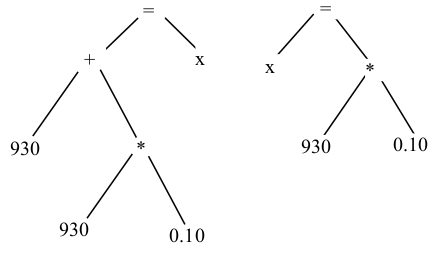
\includegraphics[height=8cm]{imgs/tree.png}
%	\end{center}
	\caption{Candidate equation tree generated with ILP}
	\label{fig:tree}
\end{figure}

\subsection{Learning}
In learning, our system will learn from the score of the equations based on the solution of the problem text, \textit{p} like ALGES. Our dataset contains problem text-solution pairs $ (w_ i ,l_ i), where, i = 1,2, ...,N$. Learning process can be divided into two parts. One is – \textbf{Local Qset Relationship Model}, and another is – \textbf{Global Equation Model}. Local Model and Global Models are trained based on the problem text, \textit{p} and solution of that problem.

\subsection{Local Qset Relationship Model}
Local Qset Relationship model is learned from the equation tree. For each equation tree, two base Qset $s_1$ and $s_2$ are used to extract the features and labeled with op as train data. If $op \in \{+, - , *, /\}$ then, $L_{local} = \theta^T f_{local}(s_1, s_2)$ where $f_{local}$ is the feature vector between the Qsets.

\subsection{Features in Local Qset Relationship Model}
Given the richness of the textual possibilities for indicating a math operation, the features are designed over semantic and intertextual relationships between Qsets, as well as domain-specific lexical features. The feature vector includes three main feature categories (Table \ref{tab:landg}).

First, single set features include syntactic and po-
sitional features of individual Qsets. For example,
they include indicator features for whether elements
of a short lexicon of math-specific terms such as ‘add’ and ‘times’ appear in the vicinity of the set
reference in the text. Also, following \cite{1}, we include a vector that captures the distance between the verbs associated with each Qset and a small collection of verbs found to be useful
in categorizing arithmetic operations in that work,
based upon their Lin Similarity\cite{31}.

Second, relationships between Qsets are described w.r.t. various Qset properties described in section 4. These include binary features like whether one Qset’s container property matches the other Qset’s entity (a strong indicator of multiplication), or
the distance between the verbs associated with each
set based upon their Lin Similarity.

Third, target quantity features check the matching
between the target Qset and the current Qset as well
as math keywords in the target sentence.
\subsection{Linear Similarity}

\noindent \textbf{Semantic similarity} is a metric defined over a set of documents or terms, where the idea of distance between them is based on the likeness of their meaning or semantic content as opposed to similarity which can be estimated regarding their syntactical representation (e.g. their string format). These are mathematical tools used to estimate the strength of the semantic relationship between units of language, concepts or instances, through a numerical description obtained according to the comparison of information supporting their meaning or describing their nature. The term semantic similarity is often confused with semantic relatedness. Semantic relatedness includes any relation between two terms, while semantic similarity only includes ``is a" relations. For example, ``car" is similar to ``bus", but is also related to ``road" and ``driving".


Our method computes the similarity between
two verbs $v_1$ and $v_2$ from the similarity between all
the senses (from WordNet) of these verbs (Equation \ref{eq:lin}). We compute the similarity between two
senses using linear similarity. The
similarity between two synsets $sv_1$ and $sv_2$ are penalized according to the order of each sense for the
corresponding verb. Intuitively, if a synset appears
earlier in the set of synsets of a verb, it is more
likely to be considered as the correct meaning.
Therefore, later occurrences of a synset should result in reduced similarity scores. The similarity
between two verbs $v_1$ and $v_2$ is the maximum similarity between two synsets of the verbs:

\begin{equation}
sim(v_1, v_2) = \max_{sv:synset(v)}^{} {lin-sim(sv_1, sv_2)\over \log(p_1+p_2)}
\label{eq:lin}
\end{equation}
where $sv_1$ , $sv_2$ are two synsets, $p_1$ , $p_2$ are the position of each synset match, and $lin-sim$ is the linear similarity.


\subsection{Global Equation Model}
Our system train global equation model to score the equation trees as in ALGES. $G_{global}= \gamma^T f_{global}(p, t)$ where  $f_{global}$   is the feature vector capturing the trees, t and the problem text, p. Root node will set based on the local model's prediction of \textit{left} and \textit{right} of the equal operator.
\subsection{Features in Global Equation Model}
Features $f$ global are explained in Table \ref{tab:landg}. They
include the number of violated soft constraints in the
ILP, the probabilities of the left and right subtrees of
the root as provided by the local model, and global
lexical features. Additionally, the three local feature
sets are applied to the left and right Qsets.

\begin{table}[H]
	\caption{Features used for Local and Global Model \cite{3}}
	\begin{center}
	\fbox{
		\begin{minipage}{0.70\textwidth}
			\begin{enumerate}
				\item \textbf{Single Qset Features (Qset A)}
				\begin{itemize}
					\item What argument of its governing verb A?
					\item Is A a subset of another set?
					\item Is A a compound?
					\item Math keywords found in the context of A?
					\item Verb Lin Distance from known verb categories?
				\end{itemize}
				\item \textbf{Relational features between Qsets}
				\begin{itemize}
					\item Entity Match
					\item Adjective Overlap
					\item Location Match
					\item Distance in text
					\item Lin Similarity
				\end{itemize}
				\item \textbf{Target Qset Features}
				\begin{itemize}
					\item Which one is target Qset?
					\item Entity Matched with target entity?
				\end{itemize}
				
				\item \textbf{Root Node Features}
				\begin{itemize}
					\item Number of ILP constraints violated by equation
					\item Scores of left and right subtrees of root
				\end{itemize}
				
				
			\end{enumerate}
		\end{minipage}
	}
	
\end{center}
\label{tab:landg}
\end{table}

\subsection{Inference}
The inference is the testing steps in Figure \ref{fig:flowchart} In inference for a problem text, \textit{P} firstly \textit{ILP(p)} generates the candidate equations. On the candidate equations, the score is calculated from local Qset Relationship model and Global Equation Model. Moreover, the final score for a candidate equation is calculated through Equation \ref{eq:main}. In ablation study ALGES shows that Global Model Score has better impact than Local Relationship Model.

\begin{equation}
	p(t|p) = (\alpha \times \prod_{t_i \in t} L_{local}(t_i | p) ) + (\beta \times G_{global}(t|p))
	\label{eq:main}
\end{equation}

Where $t_i$ is the subtree and $t$ are the roots of the equation, $\alpha$ is the bias for \textbf{Local Model Score}, $\beta$ is the bias for the \textbf{Global model score} and $\beta = (1 - \alpha)$. Among all the scores, the candidate equation with the highest score is selected for the final equation.

\section{Classifier} Choosing and designing effective classifier is a crucial step in prediction. For prediction for a operator and prediction an equation tree correct or incorrect, we have used Random Forest (RF). In this study, we found RF more useful for prediction of operator from local and global model. Here we have discussed in brief.

\subsection{Random Forests}
\textbf{Random forests} or \textbf{random decision forests} are an ensemble learning method for classification, regression and other tasks, that operate by constructing a multitude of decision trees at training time and outputting the class that is the mode of the classes (classification) or mean prediction (regression) of the individual trees. Random decision forests correct for decision trees' habit of over-fitting to their training set.
\subsubsection{Features of Random Forests}
We assume that the user knows about the construction of single classification trees. Random Forests grows many classification trees. To classify a new object from an input vector, put the input vector down each of the trees in the forest. Each tree gives a classification, and we say the tree ``votes" for that class. The forest chooses the classification having the most votes (over all the trees in the forest).
\begin{itemize}
	\item It is unexcelled in accuracy among current algorithms.
	\item It runs efficiently on large data bases.
	\item It can handle thousands of input variables without variable deletion.
	\item It gives estimates of what variables are important in the classification.
	\item It generates an internal unbiased estimate of the generalization error as the forest building progresses.
	\item It has an effective method for estimating missing data and maintains accuracy when a large proportion of the data are missing.
	\item It has methods for balancing error in class population unbalanced data sets.
	\item Generated forests can be saved for future use on other data.
	\item Prototypes are computed that give information about the relation between the variables and the classification.
	\item It computes proximities between pairs of cases that can be used in clustering, locating outliers, or (by scaling) give interesting views of the data.
	\item The capabilities of the above can be extended to unlabeled data, leading to unsupervised clustering, data views and outliers detection.
	\item It offers an experimental method for detecting variable interactions.
\end{itemize}
\subsubsection{Algorithm of Random Forest}
Decision trees are a popular method for various machine learning tasks. Tree learning ``come closest to meeting the requirements for serving as an off-the-shelf procedure for data mining", because it is invariant under scaling and various other transformations of feature values, is robust to inclusion of irrelevant features, and produces inspectable models. However, they are seldom accurate.

In particular, trees that are grown very deep tend to learn highly irregular patterns: they overfit their training sets, i.e. have low bias, but very high variance. Random forests are a way of averaging multiple deep decision trees, trained on different parts of the same training set, with the goal of reducing the variance. This comes at the expense of a small increase in the bias and some loss of interpretability, but generally greatly boosts the performance in the final model.

\subsubsection{Tree bagging}
The training algorithm for random forests applies the general technique of bootstrap aggregating, or bagging, to tree learners. Given a training set $X = x_1, ..., x_n$ with responses $Y = y_1, ..., y_n$, bagging repeatedly (B times) selects a random sample with replacement of the training set and fits trees to these samples:

For $b = 1, ..., B:$
\begin{enumerate}
	\item Sample, with replacement, $n$ training examples from $X$, $Y$; call these $X_b$, $Y_b$.
	\item Train a classification or regression tree $f_b$ on $X_b$, $Y_b$.
\end{enumerate}

After training, predictions for unseen samples $x'$ can be made by averaging the predictions from all the individual regression trees on $x'$:
\begin{equation}
{\displaystyle {\hat {f}}={\frac {1}{B}}\sum _{b=1}^{B}f_{b}(x')} 
\end{equation}
or by taking the majority vote in the case of classification trees.

This bootstrapping procedure leads to better model performance because it decreases the variance of the model, without increasing the bias. This means that while the predictions of a single tree are highly sensitive to noise in its training set, the average of many trees is not, as long as the trees are not correlated. Simply training many trees on a single training set would give strongly correlated trees (or even the same tree many times, if the training algorithm is deterministic); bootstrap sampling is a way of de-correlating the trees by showing them different training sets.

Additionally, an estimate of the uncertainty of the prediction can be made as the standard deviation of the predictions from all the individual regression trees on x':
\begin{equation}
{\displaystyle \sigma ={\sqrt {\frac {\sum _{b=1}^{B}(f_{b}(x')-{\hat {f}})^{2}}{B-1}}}.}
\end{equation}

The number of samples/trees, B, is a free parameter. Typically, a few hundred to several thousand trees are used, depending on the size and nature of the training set. An optimal number of trees B can be found using cross-validation, or by observing the out-of-bag error: the mean prediction error on each training sample $x_i$, using only the trees that did not have $x_i$ in their bootstrap sample. The training and test error tend to level off after some number of trees have been fit.

\subsubsection{From bagging to random forests}
The above procedure describes the original bagging algorithm for trees. Random forests differ in only one way from this general scheme: they use a modified tree learning algorithm that selects, at each candidate split in the learning process, a random subset of the features. This process is sometimes called ``feature bagging". The reason for doing this is the correlation of the trees in an ordinary bootstrap sample: if one or a few features are very strong predictors for the response variable (target output), these features will be selected in many of the B trees, causing them to become correlated.

Typically, for a classification problem with $p$ features, $\sqrt{p}$ (rounded down) features are used in each split. For regression problems the inventors recommend $p/3$ (rounded down) with a minimum node size of 5 as the default.



\section{Conclusion}
In PWPS, score is generated from two different model. That are called as score from Local Qset Relation Model score and Global Equation Model Score. And the final decision is made based on these score which is in the inference.
\end{document}
